%%%%%%%%%%%%%%%%%%%%%%%%%%%%%%%%%%%%%%%%%%%%%%%%%%%%%%%%%%%%%%%%%%%%%%%%%%%%%%%%%
%
% Purpose:  Conceptual part of Product Spec for the SolarBeta model
%
% 
%
%%%%%%%%%%%%%%%%%%%%%%%%%%%%%%%%%%%%%%%%%%%%%%%%%%%%%%%%%%%%%%%%%%%%%%%%%%%%%%%%


%\section{Conceptual Design}

The Solar Beta angle, $\beta$, is the angle between the Sun-vector (the vector from the center of Earth to Sun), and the projection of the Sun-vector onto the orbital plane.  An alternative view is to consider $\beta$ as $\pi /2 - \alpha$, where $\alpha$ is the angle between the orbital angular momentum vector and the Sun vector.  See Figure~\ref{fig:solarbetaintro} for a graphical representation.

\begin{figure}[htp]
\begin{center}
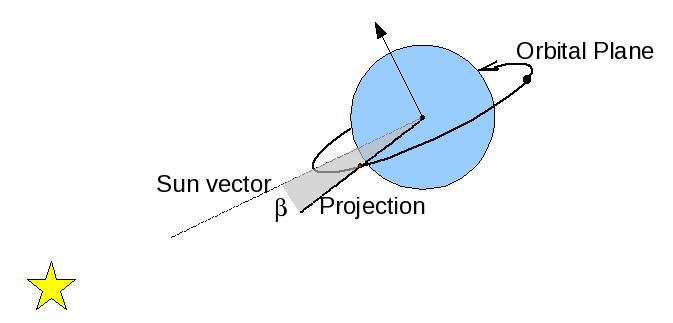
\includegraphics[width=5in]{figures/solar_beta.jpg}
\caption{The definition of the Solar Beta angle.  The arrow represents the orbital angular momentum vector.  Note that the position of the vehicle (upper right) on the orbit is of no consequence to the determination of the Solar Beta angle.}
\label{fig:solarbetaintro}
\end{center}
\end{figure}

$\beta$ is positive when the Sun-vector is above the orbital plane (i.e., when it is aligned in the same general sense as the orbital angular momentum vector, also interpreted as when the dot product of these two vectors is positive), zero when the Sun-vector lies in the orbital plane, and negative when the Sun-vector lies below the orbital plane.  $\beta \in \left[ -\frac{\pi}{2}, \frac{\pi}{2} \right]$.  

$\beta$ is affected by orbital precession, and by the orbital motion of Earth with respect to Sun.  It is not directly affected by the vehicle's position on its orbit.

As an illustration, consider a vehicle in an equatorial orbit.  At the equinoxes, the Sun-vector lies in the orbital plane, and $\beta = 0$.  In the Northern summer (April - September), the sun lies above the equator, hence above the orbit (assuming that the orbit is in the same sense as Earth's rotation), and $\beta > 0$, reaching a peak at the solstice.  In the Southern summer (October - March), the sun is below the equator, hence below the orbit, and $\beta < 0$, reaching a minimum at the solstice.

The effect of precession and time of year can be seen in Figure~\ref{fig:solarbetaISS}, which shows the typical variation with time of the Solar beta angle for a vehicle in an orbit comparable to that of the International Space Station.

\begin{figure}[htp]
\begin{center}
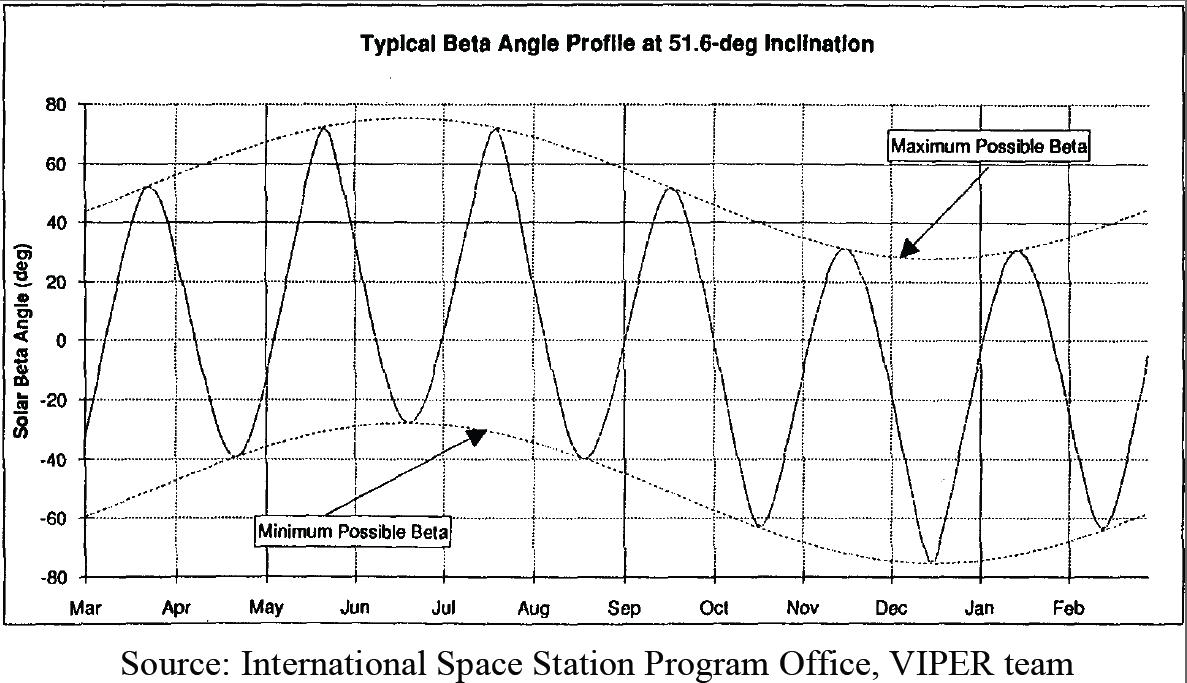
\includegraphics[width=5in]{figures/solar_beta_iss.jpg}
\caption{The variation with time of the Solar Beta angle for an orbit with inclination of 51.6 degrees.  The high frequency oscillation is due to precession, and the long period variation due to Earth's motion around Sun.}
\label{fig:solarbetaISS}
\end{center}
\end{figure}

